%% abtex2-modelo-include-comandos.tex, v-1.9.6 laurocesar
%% Copyright 2012-2016 by abnTeX2 group at http://www.abntex.net.br/ 
%%
%% This work may be distributed and/or modified under the
%% conditions of the LaTeX Project Public License, either version 1.3
%% of this license or (at your option) any later version.
%% The latest version of this license is in
%%   http://www.latex-project.org/lppl.txt
%% and version 1.3 or later is part of all distributions of LaTeX
%% version 2005/12/01 or later.
%%
%% This work has the LPPL maintenance status `maintained'.
%% 
%% The Current Maintainer of this work is the abnTeX2 team, led
%% by Lauro César Araujo. Further information are available on 
%% http://www.abntex.net.br/
%%
%% This work consists of the files abntex2-modelo-include-comandos.tex
%% and abntex2-modelo-img-marca.pdf
%%

\chapter{Validação dos Cálculos}
	\label{calculos_exp}

	\section{Introdução}
		
		O carbono se apresenta de maneira natural principalmente na forma de grafite e diamante. Apesar de essas serem as formas alotrópicas do carbono mais abundantes na natureza, não são as únicas existentes. Atualmente já foram observadas 11 formas alotrópicas deste elemento\footnote{Grafite, Diamante, Lonsdaleite, Grafeno, Nanotubos, Fullerenos, Schwarzitas, Carbina, T-Carbon, Q-Carbon, Cyclo[18]carbon}, sendo que todas exceto grafite e diamante somente foram observadas experimentalmente nos últimos 50 anos. 
		
		Neste capítulo Diamante, Grafite e Lonsdaleite serão apresentados, explorando um pouco de sua história, aplicações industriais e aspectos estruturais. Os dados experimentais medidos para diversas propriedades diferentes serão comparados com valores calculados com diferentes funcionais, com o intuito de comparar, calibrar e determinar a melhor metodologia para fazer cálculos de novas estruturas propostas.
		
	\section{Diamante}
	
		\begin{figure}[!h]
			\centering
			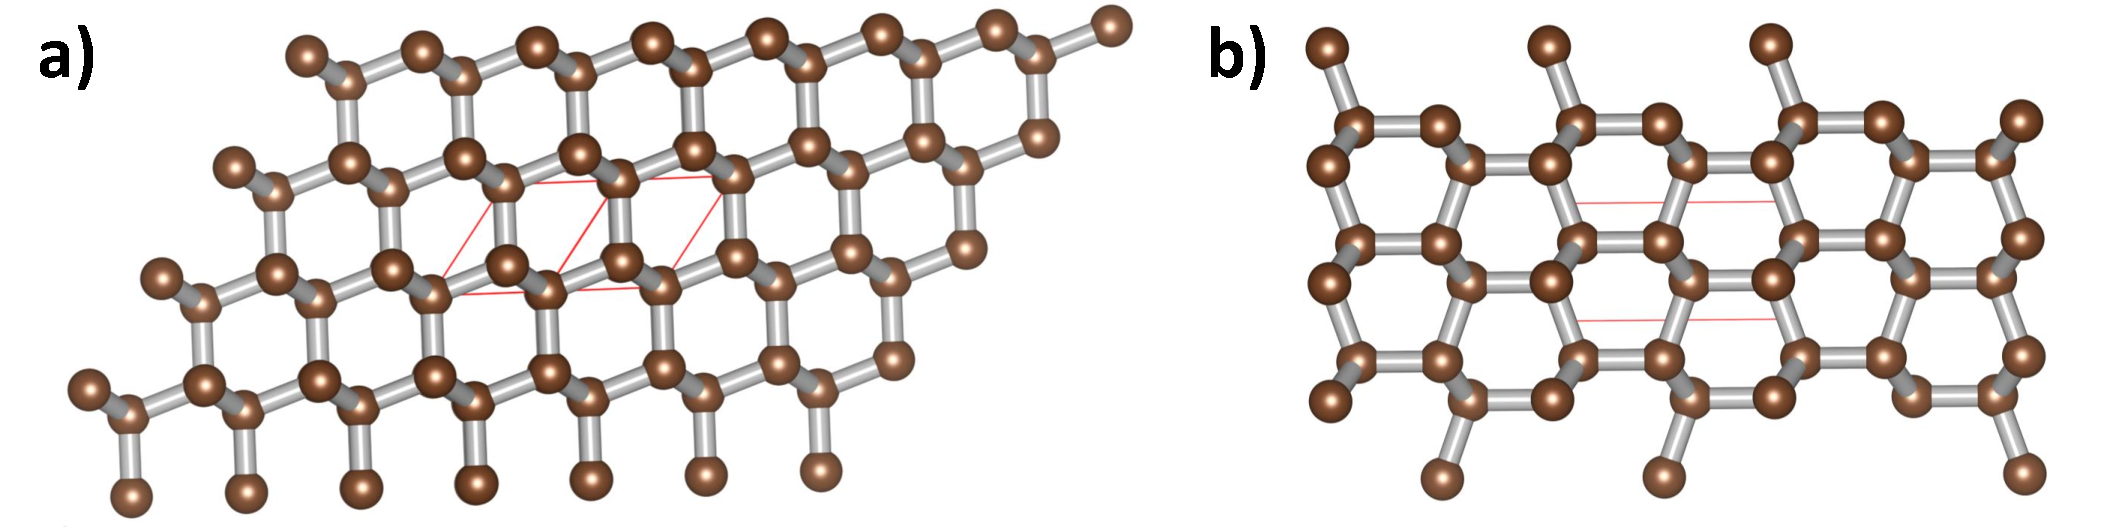
\includegraphics[width=1.\linewidth]{capitulos/fig/results0/diamante_losndaleite}
			\caption{Estrutura do a) Diamante e b) Lonsdaleite com suas respectivas células primitivas em vermelho}
			\label{diamante_lonsdaleite}
		\end{figure}

		O diamante é um sólido covalente com estrutura cúbica de face centrada formado somente por átomos de carbono com hibridação $sp^3$. Ele apresenta a maior dureza e condutividade térmica dentre os materiais minerais naturais, propriedades que são o principal foco de suas diversas aplicações comerciais. Além disso, devido a sua alta capacidade de dispersão de luz, alto índice de refração, por ser quimicamente inerte e sua alta raridade, com concentração média de partes por bilhão no manto terrestre \cite{cartigny2014diamond}, os diamantes também são amplamente utilizados como adereços e joias. O diamante é uma fase metaestável à temperatura e pressão ambiente, sendo a fase termodinamicamente mais estável do carbono somente acima de 60 kbar \cite{pierson2012handbook}. Devido a isso, sua formação natural ocorre somente em regiões com profundidade maior que 150 km, onde há pressão e temperatura suficiente para que sua estrutura seja termodinamicamente estável e sua formação ocorra em taxas apreciáveis. 
		
		Devido às suas excelentes propriedades e estrutura relativamente simples o diamante é um sólido extremamente estudado e com uma ampla gama de dados experimentais disponíveis, o que faz dessa estrutura um modelo de sólido covalente 3D excelente para calibrar e validar cálculos teóricos. 
		
		%\begin{landscape}
		\begin{table}[]
			\centering
			\caption{Comparação entre valores experimentais e calculados com diferentes funcionais para a célula primitiva do diamante.}
			\label{dados_diamante}
			\renewcommand{\arraystretch}{1.2}
			\fontfamily{lmss}\small\selectfont
			\begin{tabular}{l|ccccccc}
				\hline\hline
				& $a$ & $\rho$ & d(C-C) & \textbf{B} & E. Coeh. & \textit{Band Gap} & Freq. \\
				& (\AA{}) & (cm$^3$/g) & (\AA{}) & (GPa) & (eV/átomo) & (eV) & (cm$^{-1}$) \\ \hline
				Experimental & 3.567\textsuperscript{\cite{hom1975accurate}} & 3.523\textsuperscript{\cite{hom1975accurate}}     & 1.544\textsuperscript{\cite{hom1975accurate}}       & 442\textsuperscript{\cite{grimsditch1975brillouin}}     &  7.58\textsuperscript{\cite{greenwood2012chemistry}}     & 5.47\textsuperscript{\cite{greenwood2012chemistry}}     & 1332\textsuperscript{\cite{warren1967lattice}}         \\
				LDA          & 3.534 & 3.616     & 1.530        & 465.3   &  8.98     & 4.19     & 1321         \\
				LDA-D2       & 3.525 & 3.641     & 1.527        & 471.3   &  9.19     & 4.21     & 1337         \\
				GGA-PBE      & 3.571 & 3.504     & 1.546        & 432.9   &  7.65     & 4.18     & 1290         \\
				GGA-PBE-D2   & 3.562 & 3.529     & 1.543        & 440.8   &  7.86     & 4.19     & 1307         \\
				GGA-PBE-D3   & 3.565 & 3.521     & 1.544        & 435.3   &  7.74     & 4.19     & 1297         \\
				GGA-PBESol   & 3.555 & 3.552     & 1.539        & 449.7   &  8.32     & 4.08     & 1307         \\
				GGA-PBESol-D2& 3.547 & 3.576     & 1.536        & 449.7   &  8.45     & 4.10     & 1321         \\
				GGA-PBESol-D3& 3.552 & 3.562     & 1.538        & 451.1   &  8.30     & 4.09     & 1309         \\
				GGA-BLYP     & 3.599 & 3.422     & 1.559        & 402.0   &  6.58     & 4.46     & 1296         \\
				GGA-BLYP-D2  & 3.590 & 3.447     & 1.555        & 441.2   &  6.79     & 4.41     & 1276         \\
				GGA-BLYP-D3  & 3.588 & 3.454     & 1.554        & 409.4   &  6.75     & 4.41     & 1271         \\
				GGA-PW91     & 3.571 & 3.503     & 1.547        & 430.3   &  7.49     & 4.19     & 1289         \\
				GGA-PW91-D2  & 3.563 & 3.528     & 1.543        & 438.1   &  7.70     & 4.21     & 1306         \\
				B3LYP        & 3.567\textsuperscript{a} &           &              &         &           & 5.97     &              \\
				HSE          & 3.567\textsuperscript{a} &           &              &         &           & 5.39     &              \\ \hline\hline          
			\end{tabular}
		\textsuperscript{a}Foram utilizados os valores experimentais para o cálculo com funcionais híbridos. 
		\end{table}
	    %\end{landscape}
		
		\begin{figure}[!h]
			\centering
			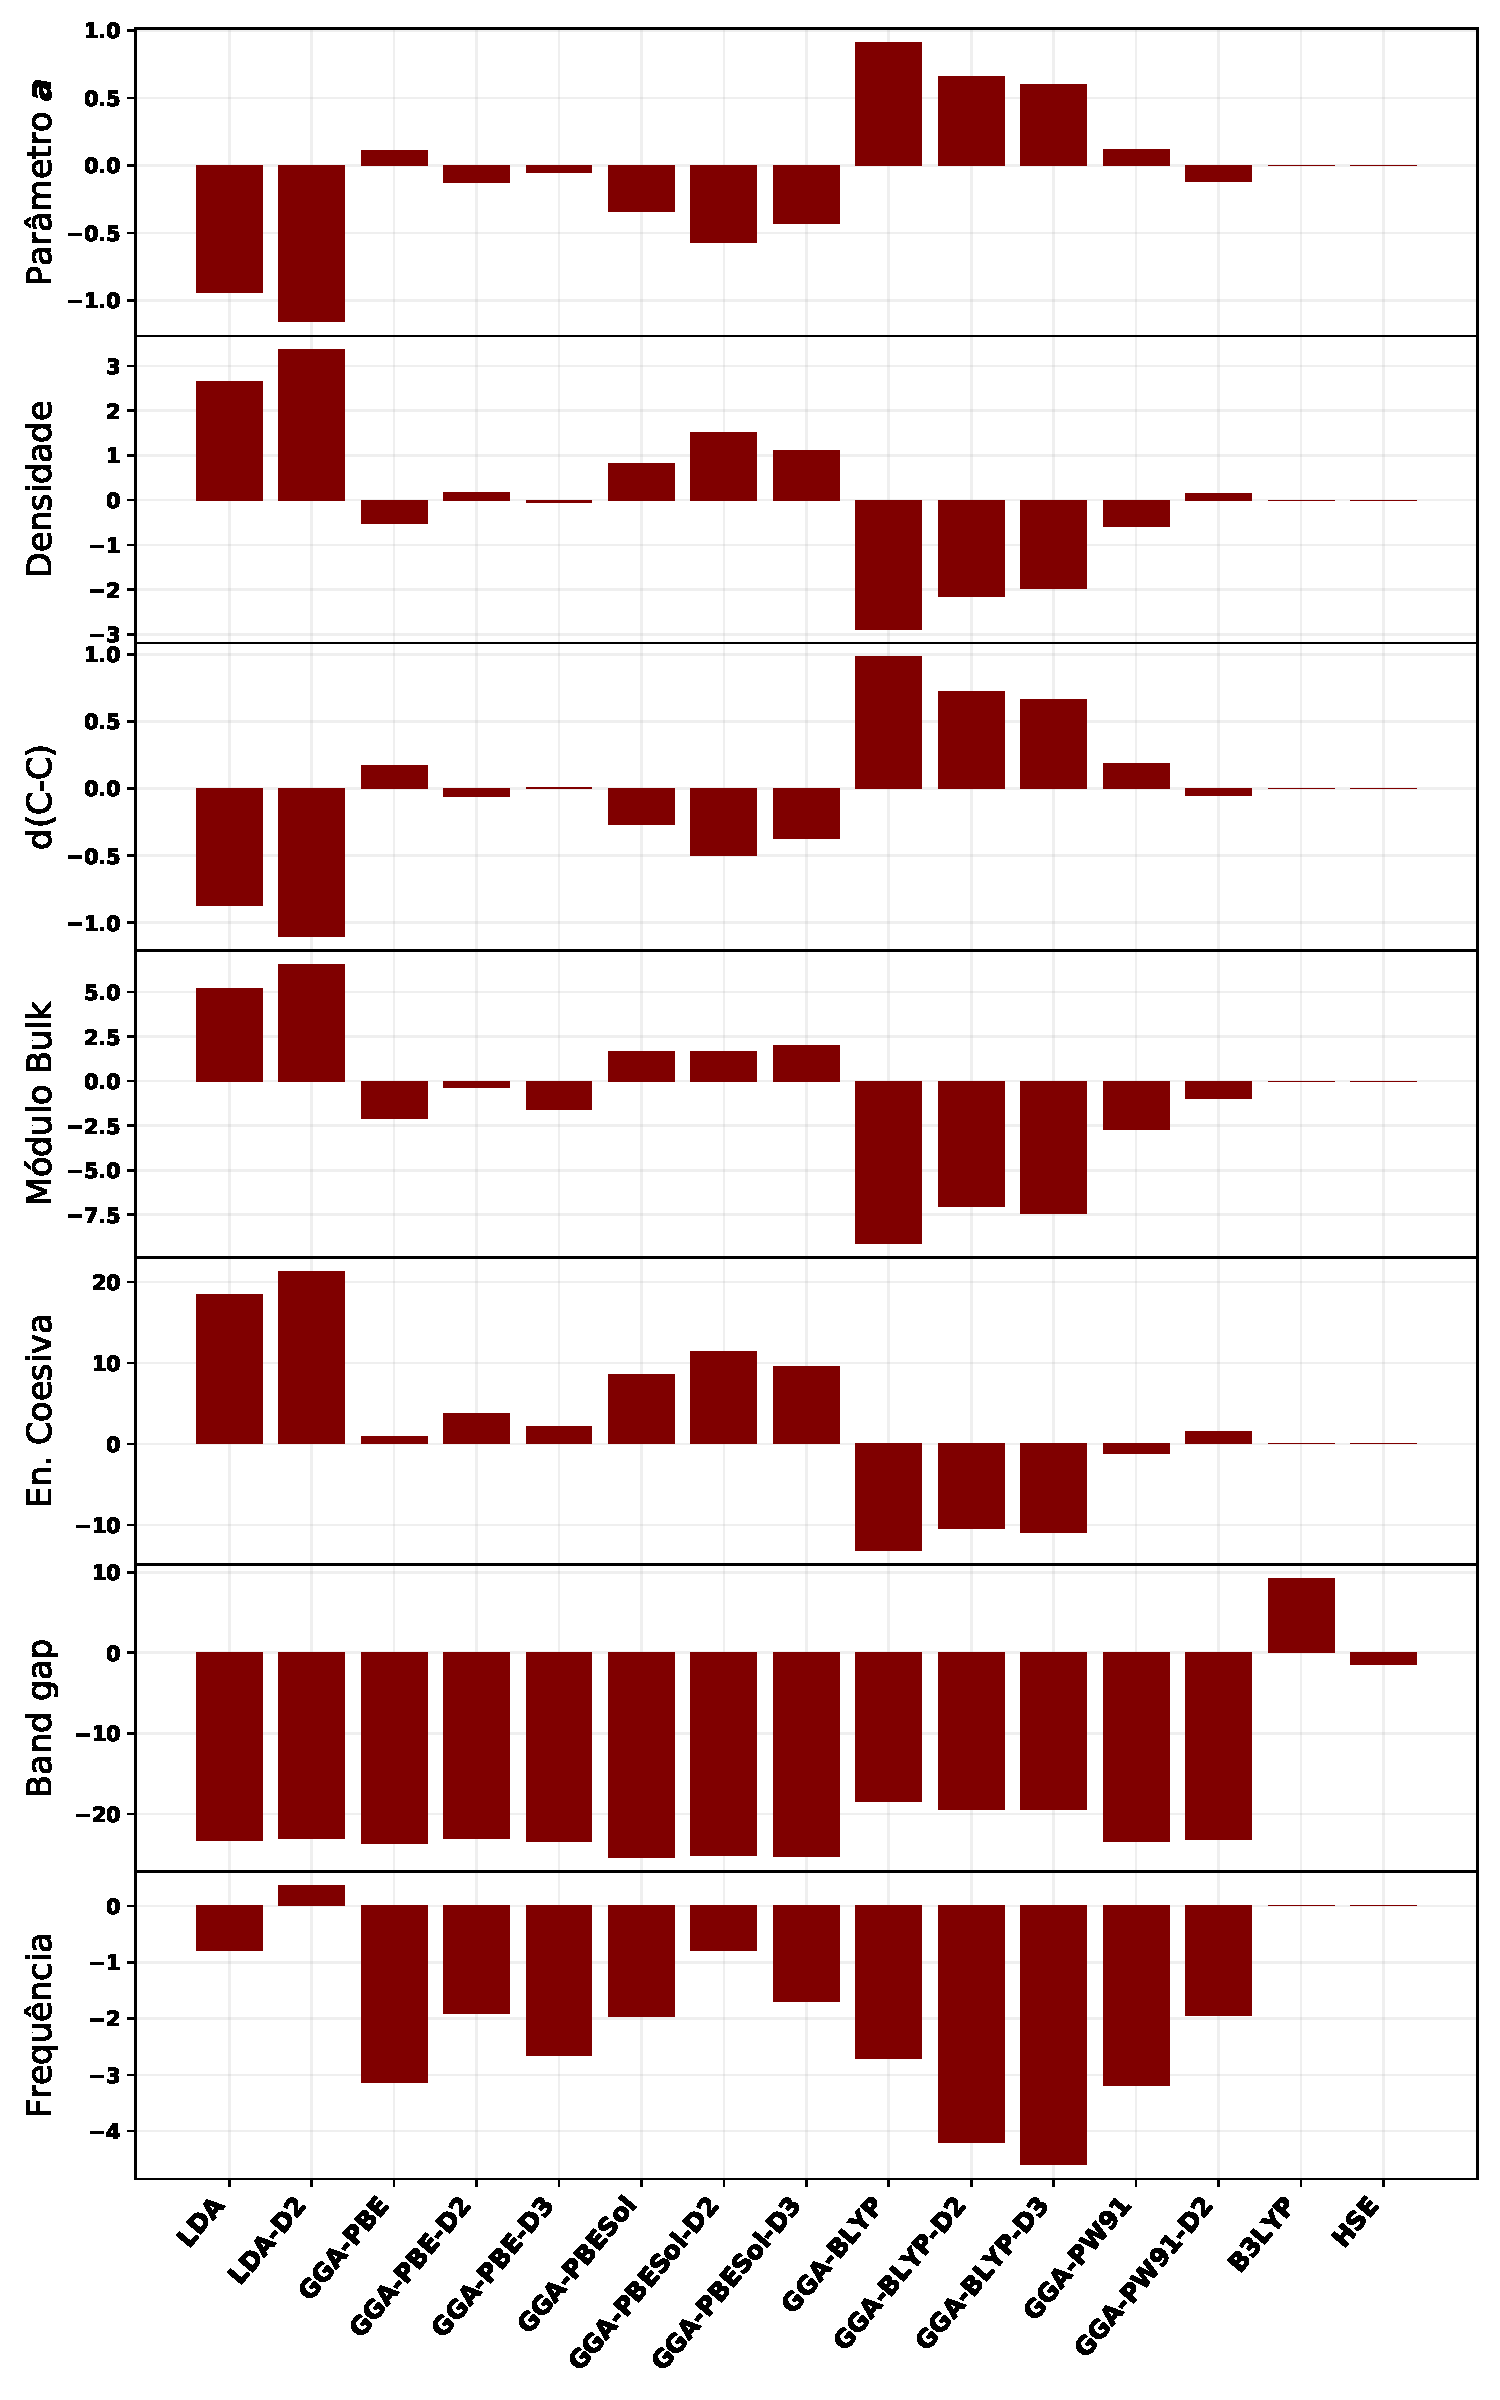
\includegraphics[width=.85\linewidth]{capitulos/fig/results0/disc_rel_diamante}
			\caption{Discrepância relativa percentual de diversas propriedades do diamante calculadas para vários funcionais.}
			\label{disc_rel_diamante}
		\end{figure}
	
		A \autoref{dados_diamante} apresenta uma comparação dos valores calculados com diferentes funcionais para diversas propriedades com seus respectivos valores experimentais. As discrepâncias relativas percentuais entre os dados experimentais e os teóricos são apresentados na \autoref{disc_rel_diamante}.
		
		As discrepâncias relativas percentuais apresentadas para o parâmetro de célula ($a$) foram menores que 0.5\% para os funcionais GGA-PBE, GGA-PBESol GGA-PW91 e na casa dos 1\% para os funcionais LDA, GGA-BLYP. A inclusão de correções de forças de dispersão não causa grande influência, o que já era esperado uma vez que a estrutura do diamante não apresenta interações dispersivas apreciáveis. Densidade, comprimento das ligações (d(C-C)) e módulo Bulk apresentaram um comportamento similar, tendo os funcionais GGA-PBE, GGA-PBESol e GGA-PW91 apresentado os melhores resultados. 
		
		Para a energia coesiva os funcionais LDA, GGA-PBESol e GGA-BLYP apresentaram diferenças percentuais acima de 10\% enquanto os funcionais GGA-PBE e GGA-PW91 apresentaram valores muito próximos do experimental. As discrepâncias relativas apresentadas para o cálculo da frequência vibracional em $\Gamma$ foram baixas, sendo todas abaixo dos 4\%. 
		
		Os valores calculados para \textit{band gap} apresentaram diferenças relativas grandes, na casa dos 20\% para todos os funcionais, sendo em todos os casos menores do que o observado experimentalmente. Esse comportamento já era esperado, devido ao conhecido problema que funcionais \textit{ab initio} apresentam em predizer energias de estados de Kohn-Sham não ocupados. Para se obter valores de \textit{band gap} mais próximo do experimental para materiais isolantes é comum a utilização de funcionais híbridos, como o B3LYP (Becke, 3 parâmetros, Lee–Yang–Parr) que apresenta três parâmetros ajustados para representar energias de atomização, potenciais de ionização, energias atômicas totais e afinidade de próton; ou HSE (Heyd–Scuseria–Ernzerhof), em que o funcional de troca-correlação utiliza uma função de erro sobre o potencial de Coulomb para calcular a porção de troca da energia total. \cite{heyd2003hybrid} É possível notar que esses funcionais apresentam erros muito menores do que os anteriores, com destaque para o funcional HSE que apresentou discrepância relativa de 1,5\%. 
 	     
 	\section{Lonsdaleite}
 	
 		Lonsdaleite, também conhecido como diamante hexagonal, é um alótropo de carbono composto somente por átomos $sp^3$, com célula unitária hexagonal e grupo espacial P6\textsubscript{3}/mmc que apresenta propriedades muito semelhantes ao diamante. Essa fase foi identificada pela primeira vez em 1967 a partir de fragmentos dos meteoritos Canyon Diablo e Goalpara\cite{hanneman1967hexagonal} e foi sintetizada em laboratório sob alta pressão de maneira tanto estática quando sobe \textit{shock} no mesmo ano \cite{frondel1967lonsdaleite}. Seu nome é dado em homenagem à Professora Kathleen Lonsdale, cristalógrafa que determinou a estrutura do benzeno em 1929 por difração de raios-X \cite{lonsdale1929structure} e fez diversas contribuições aos conhecimentos sobre a estrutura do grafite e do diamante. 
 		
 		Alguns trabalhos indicam que esse material pode possuir dureza maior do que a apresentada pelo diamante \cite{pan2009harder}, apesar dessa propriedade nunca ter sido mensurada experimentalmente, e até mesmo que essa fase pode ser um intermediário metainstável da transição do grafite para o diamante \cite{fayos1999possible, kraus2016nanosecond}. Há, ainda hoje, certa controvérsia sobre a sua real existência como um material discreto, e apesar de diversos dados experimentais existirem \citeauthor{nemeth2014lonsdaleite} sugerem que essa fase na verdade pode ser resultado de defeitos, geminações e falhas de empilhamento do diamante cúbico. 
 		
 		\begin{table}[!h]
 			\centering
 			\caption{Comparação entre valores experimentais e calculados com diferentes funcionais para o Lonsdaleite.}
 			\label{lonsdaleite}
 			\renewcommand{\arraystretch}{1.1}
 			\fontfamily{lmss}\tiny\selectfont
 			\begin{tabular}{l|ccccccccc}
 				\hline\hline
 				& a     & c     & Dens. & d1(C-C) & d2(C-C) & B & E. Coeh. & \textit{Band Gap}. & Freq. \\
 				& (\AA{}) & (\AA{}) & (cm$^3$/g) & (\AA{}) & (\AA{}) & (GPa) & (eV/átomo) & (eV) & (cm$^{-1}$)\\ \hline
 				Experimental  & 2.522 \textsuperscript{\cite{bundy1967hexagonal}} & 4.119\textsuperscript{\cite{bundy1967hexagonal}} & 3.52\textsuperscript{\cite{bundy1967hexagonal}} & 1.545\textsuperscript{\cite{bundy1967hexagonal}} & 1.543\textsuperscript{\cite{bundy1967hexagonal}} &  -\textsuperscript{a}  & -\textsuperscript{a}     &  -\textsuperscript{a}  & 1324\textsuperscript{\cite{misra2006hexagonal}} \\
 				LDA           & 2.485 & 4.138 & 3.61 & 1.549 & 1.526 & 465 &  8.95  & 3.0 & 1326 \\
 				LDA-D2        & 2.485 & 4.138 & 3.61 & 1.549 & 1.526 & 460 &  8.95  & 3.0 & 1331 \\
 				PBE       & 2.511 & 4.179 & 3.50 & 1.565 & 1.542 & 433 &  7.63  & 3.4 & 1295 \\
 				PBE-D2    & 2.504 & 4.167 & 3.53 & 1.561 & 1.537 & 437 &  7.83  & 3.4 & 1313 \\
 				PBE-D3    & 2.507 & 4.172 & 3.51 & 1.563 & 1.539 & 436 &  7.72  & 3.4 & 1302 \\
 				PBESol    & 2.500 & 4.162 & 3.54 & 1.558 & 1.535 & 450 &  8.21  & 3.1 & 1310 \\
 				PBESol-D2 & 2.493 & 4.149 & 3.57 & 1.554 & 1.531 & 453 &  8.42  & 3.1 & 1327 \\
 				PBESol-D3 & 2.497 & 4.157 & 3.55 & 1.557 & 1.533 & 452 &  8.28  & 3.1 & 1315 \\
 				BLYP      & 2.531 & 4.214 & 3.41 & 1.580 & 1.554 & 402 &  6.55  & 3.9 & 1264 \\
 				BLYP-D2   & 2.524 & 4.202 & 3.44 & 1.576 & 1.549 & 406 &  6.76  & 3.8 & 1282 \\
 				BLYP-D3   & 2.523 & 4.198 & 3.45 & 1.574 & 1.548 & 405 &  6.72  & 3.8 & 1277 \\
 				PW91      & 2.511 & 4.181 & 3.49 & 1.566 & 1.542 & 430 &  7.46  & 3.4 & 1294 \\
 				PW91-D2   & 2.504 & 4.168 & 3.52 & 1.562 & 1.537 & 434 &  7.67  & 3.4 & 1312 \\
 				B3LYP         & 2.485 & 4.138 &      &       &       &     &  5.09  &     &      \\
 				HSE           & 2.485 & 4.138 &      &       &       &     &  4.36  &     &      \\ \hline\hline           
 			\end{tabular}
 		\begin{flushleft}
 			\textsuperscript{a}Não existem dados experimentais relatados para essas propriedades.
 		\end{flushleft}
 		\end{table}
 	
 		\begin{figure}[!h]
	 		\centering
	 		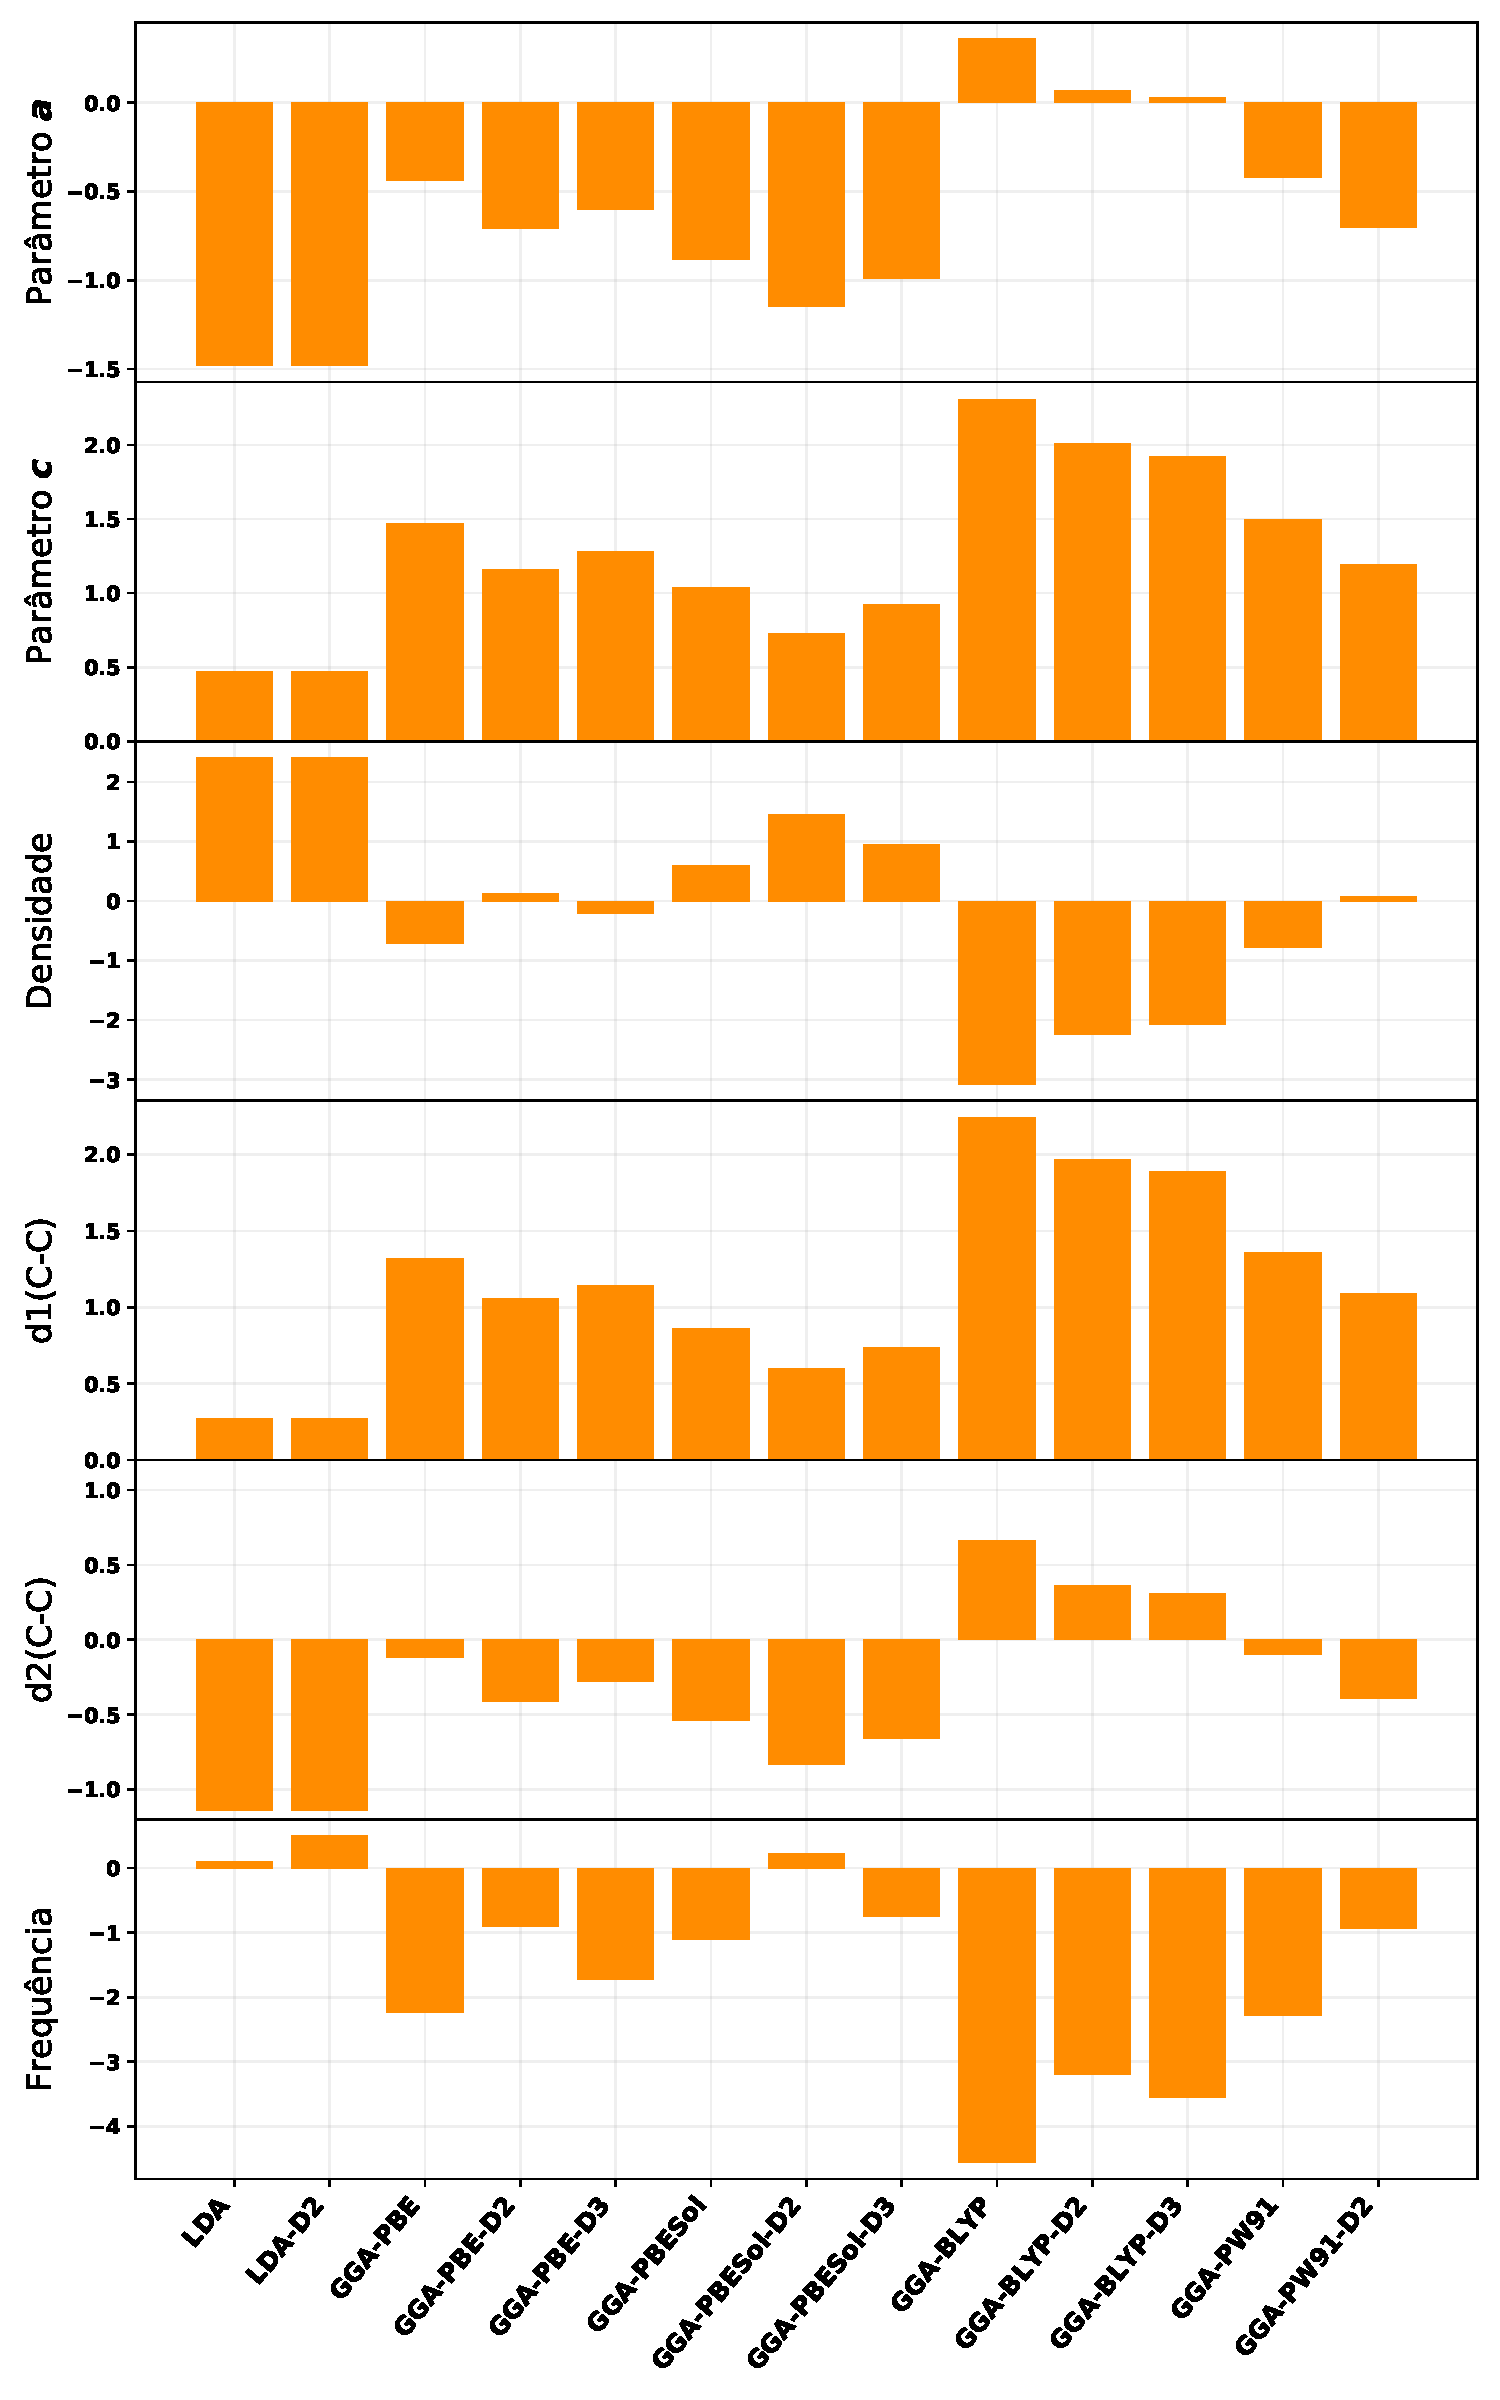
\includegraphics[width=.85\linewidth]{capitulos/fig/results0/disc_rel_lonsdaleite}
	 		\caption{Discrepância relativa percentual de diversas propriedades do diamante calculadas para vários funcionais.}
	 		\label{disc_rel_lonsdaleite}
	 	\end{figure}
 		
 		A \autoref{disc_rel_lonsdaleite} apresenta as discrepâncias relativas entre os dados experimentais, quando existem, com os valores calculados para o Lonsdaleite, apresentados na \autoref{lonsdaleite}. Os funcionais apresentaram performances similares aos resultados obtidos para o diamante. As discrepâncias relativas dos parâmetros $a$ e $c$ da célula unitária ficaram em torno de 1 e 2\%, respectivamente, tendo os funcionais GGA-PBE, GGA-PBESol e GGA-PW91 apresentado os melhores resultados. A densidade e os comprimentos das ligações seguiram o mesmo padrão. É possível observar que assim como no diamante as correções de energia de dispersão não apresentam uma diferença significativa, uma consequência direta da presença de somente átomos de carbono $sp^3$ nessa estrutura. Assim como para o diamante, o funcional LDA foi o que apresentou melhores resultados para o cálculo da frequência vibracional. Entretanto, os funcionais GGA-PBE GGA-PBESol também apresentaram excelentes resultados.
 		
 		Devido à escassez de dados experimentais, somente dados derivados da estrutura de raios-X, como parâmetros de célula e comprimentos de ligação, e dados derivados de espectroscopia Ramam, como frequência, foram utilizados para comparação. Não obstante, os valores de propriedades como módulo Bulk, energia coesiva e \textit{band gap} também são apresentados na \autoref{lonsdaleite}, de modo que possa ser feita uma comparação relativa com outros alótropos caso seja de interesse futuro.
 		
 	
	\section{Grafite}

		Nomeado pelo geólogo alemão Abraham Gottlob Werner em 1789 \cite{frohs2000carbon}, o grafite é encontrado naturalmente na forma de um mineral cinza com aspecto metálico, sendo o alótropo termodinamicamente estável do carbono à temperatura e pressão ambientes. Ele pode existir em duas formas cristalinas: hexagonal ($\alpha$) ou romboédrica ($\beta$). Ambas as formas são constituídas por camadas de átomos de carbono apresentando hibridação $sp^2$ ligados covalentemente por ligações $\sigma$ e $\pi$ entre si com distância de aproximadamente 1,42 \AA{}, em uma rede hexagonal. Como todas as ligações covalentes estão no mesmo plano, a interação entra as camadas se dá por ligações do tipo van der Waals. A forma hexagonal, também conhecida como forma alfa, é formada por um empilhamento eclipsado AB (\autoref{empilhamento_grafite}-c)) com uma distância interplano de 3.35 \AA{}. A forma romboédrica, também conhecida como forma beta, é bastante similar à forma hexagonal, entretanto o empilhamento das folhas segue um padrão eclipsado ABC, como mostrado na \autoref{empilhamento_grafite}-c). O grafite natural é uma mistura de ambas as formas, sendo em geral formada majoritariamente de grafite hexagonal.\cite{burchell1999carbon}	
		
		\begin{figure}[!h]
			\centering
			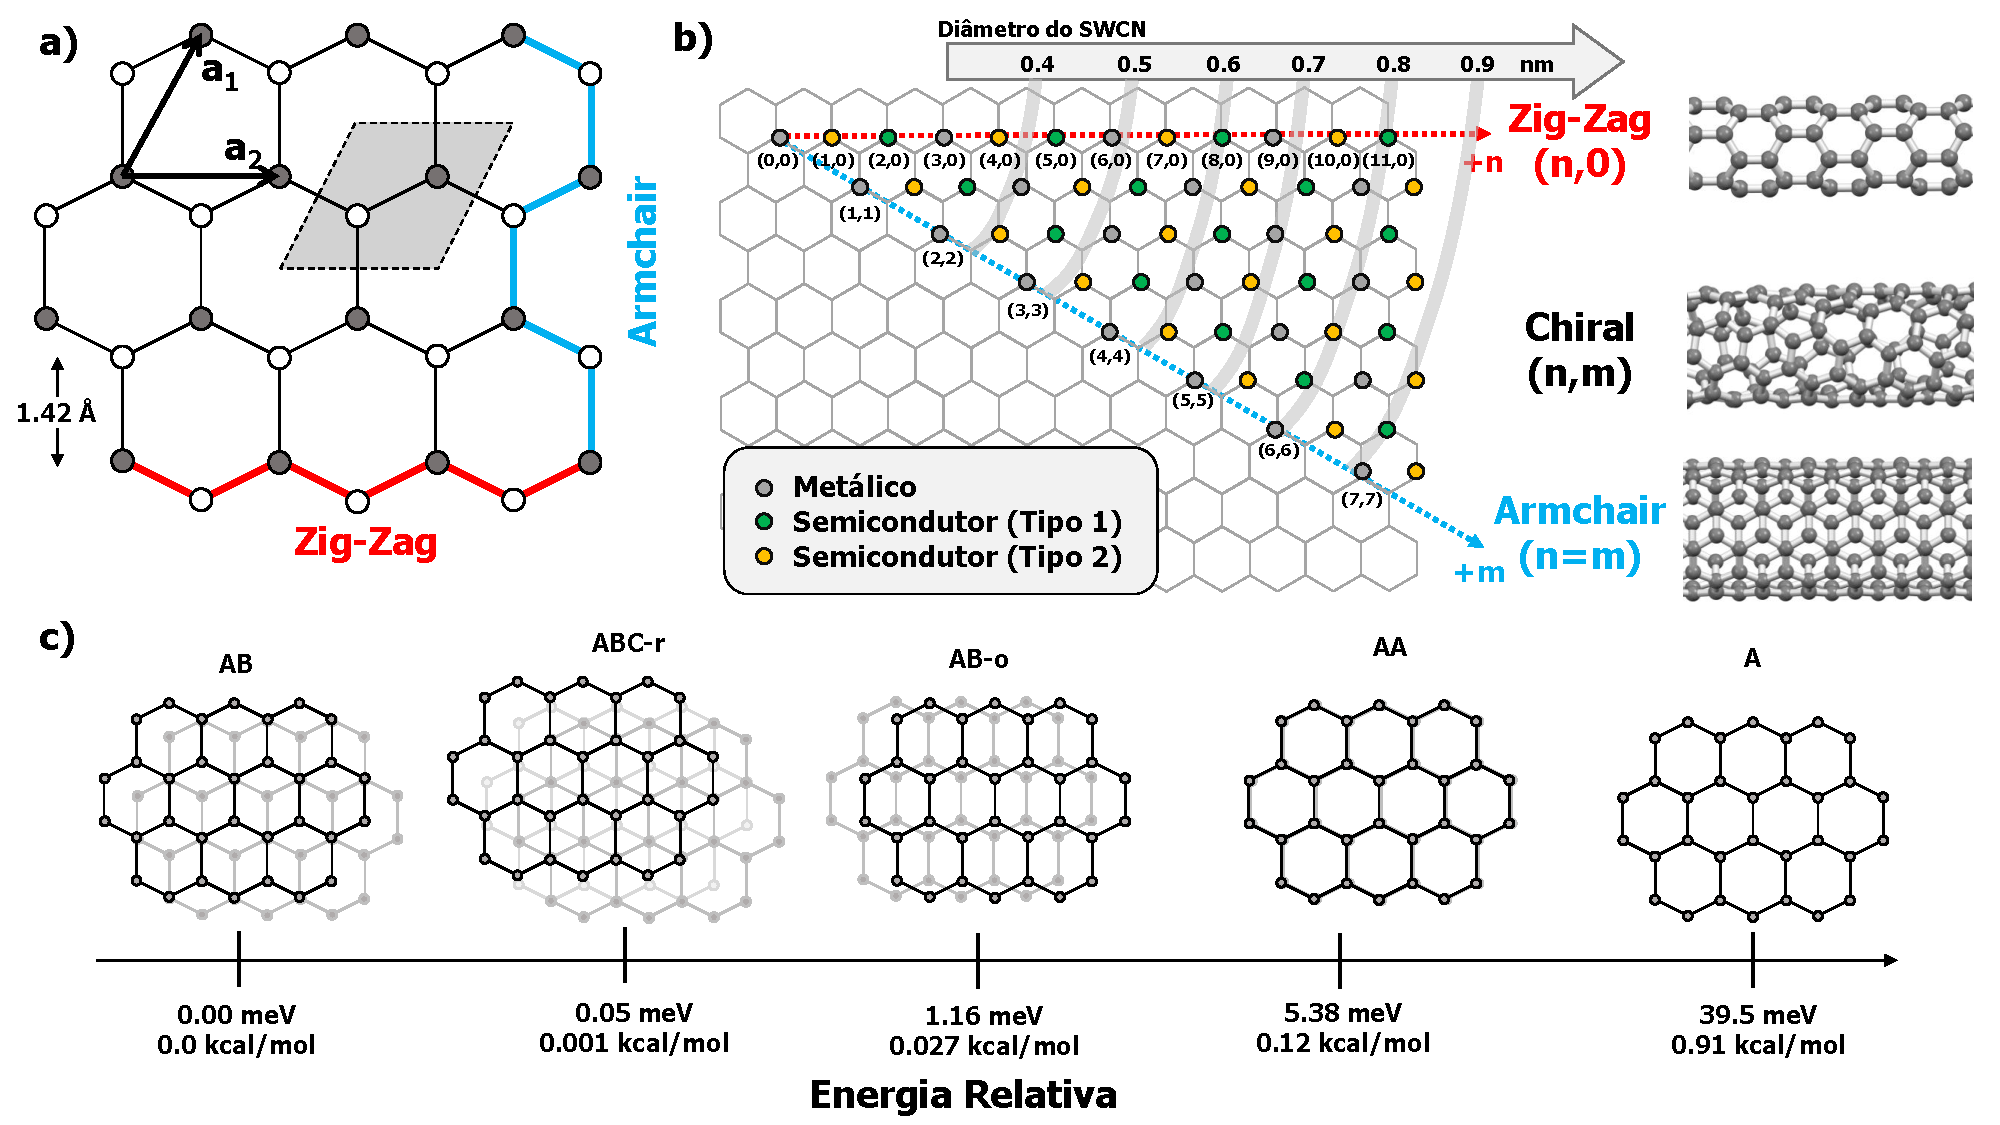
\includegraphics[width=1\linewidth]{capitulos/fig/results0/empilhamento_grafite}
			\caption{\textbf{a)} Representação da rede hexagonal do grafeno; \textbf{b)} Representação das direções principais de formação de nanotubos; \textbf{c)} Possíveis empilhamentos do grafite e suas energias relativas calculadas em nível DFT-PBE-D3.}
			\label{empilhamento_grafite}
		\end{figure}
	
		\begin{table}[]
			\centering
			\caption{Comparação entre valores experimentais e calculados com diferentes funcionais para grafite AB.}
			\label{grafite_AB}
			\renewcommand{\arraystretch}{1.2}
			\fontfamily{lmss}\tiny\selectfont
			\begin{tabular}{l|ccccccc}
				\hline\hline
							  & a     & c     & Dens. & d(C-C) & B & E. Coeh. & E. Exfol. \\
				 			  & (\AA{}) & (\AA{}) & (cm$^3$/g) & (\AA{}) & (GPa) & (eV/átomo) & (meV/átomo)\\ \hline
				Experimental  & 2.456\textsuperscript{\cite{wyckoff1963crystal}} & 6.696\textsuperscript{\cite{wyckoff1963crystal}} &   2.281\textsuperscript{\cite{wyckoff1963crystal}}       &      1.418\textsuperscript{\cite{wyckoff1963crystal}}        & 286\textsuperscript{\cite{furthmuller1994ab}} &     7.75\textsuperscript{\cite{greenwood2012chemistry}}            &     22.8\textsuperscript{\cite{benedict1998microscopic}}      \\
				LDA           & 2.446 & 6.618 &   2.327       &      1.412        & 292.79  &     8.97           &    30.92      \\
				LDA-D2        & 2.441 & 5.956 &   2.596       &      1.409        & 328.56  &     9.11           &   119.72      \\
				GGA-PBE       & 2.465 & 8.069 &   1.878       &      1.423        & 228.46  &     7.79           &     2.03      \\
				GGA-PBE-D2    & 2.461 & 6.419 &   2.369       &      1.421        & 287.01  &     7.90           &    59.50      \\
				GGA-PBE-D3    & 2.465 & 7.000 &   2.166       &      1.413        & 272.44  &     7.86           &    41.26      \\
				GGA-PBESol    & 2.459 & 7.162 &   2.126       &      1.420        & 263.07  &     8.25           &     5.85      \\
				GGA-PBESol-D2 & 2.455 & 6.100 &   2.506       &      1.417        & 311.32  &     8.39           &    84.98      \\
				GGA-PBESol-D3 & 2.459 & 6.645 &   2.292       &      1.420        & 291.73  &     8.32           &    41.21      \\
				GGA-BLYP      & 2.474 & 9.163 &   1.643       &      1.428        &- 184.08  &     6.89           &    -3.90      \\
				GGA-BLYP-D2   & 2.469 & 6.749 &   2.239       &      1.426        & 262.42  &     6.98           &    33.34      \\
				GGA-BLYP-D3   & 2.471 & 6.703 &   2.252       &      1.426        & 284.09  &     7.02           &    57.00      \\
				GGA-PW91      & 2.465 & 8.675 &   1.748       &      1.423        & 212.41  &     7.64           &     1.89      \\
				GGA-PW91-D2   & 2.460 & 6.357 &   2.395       &      1.420        & 289.37  &     7.74           &    54.68      \\ \hline\hline           
			\end{tabular}
		\end{table}

		\begin{figure}[!h]
			\centering
			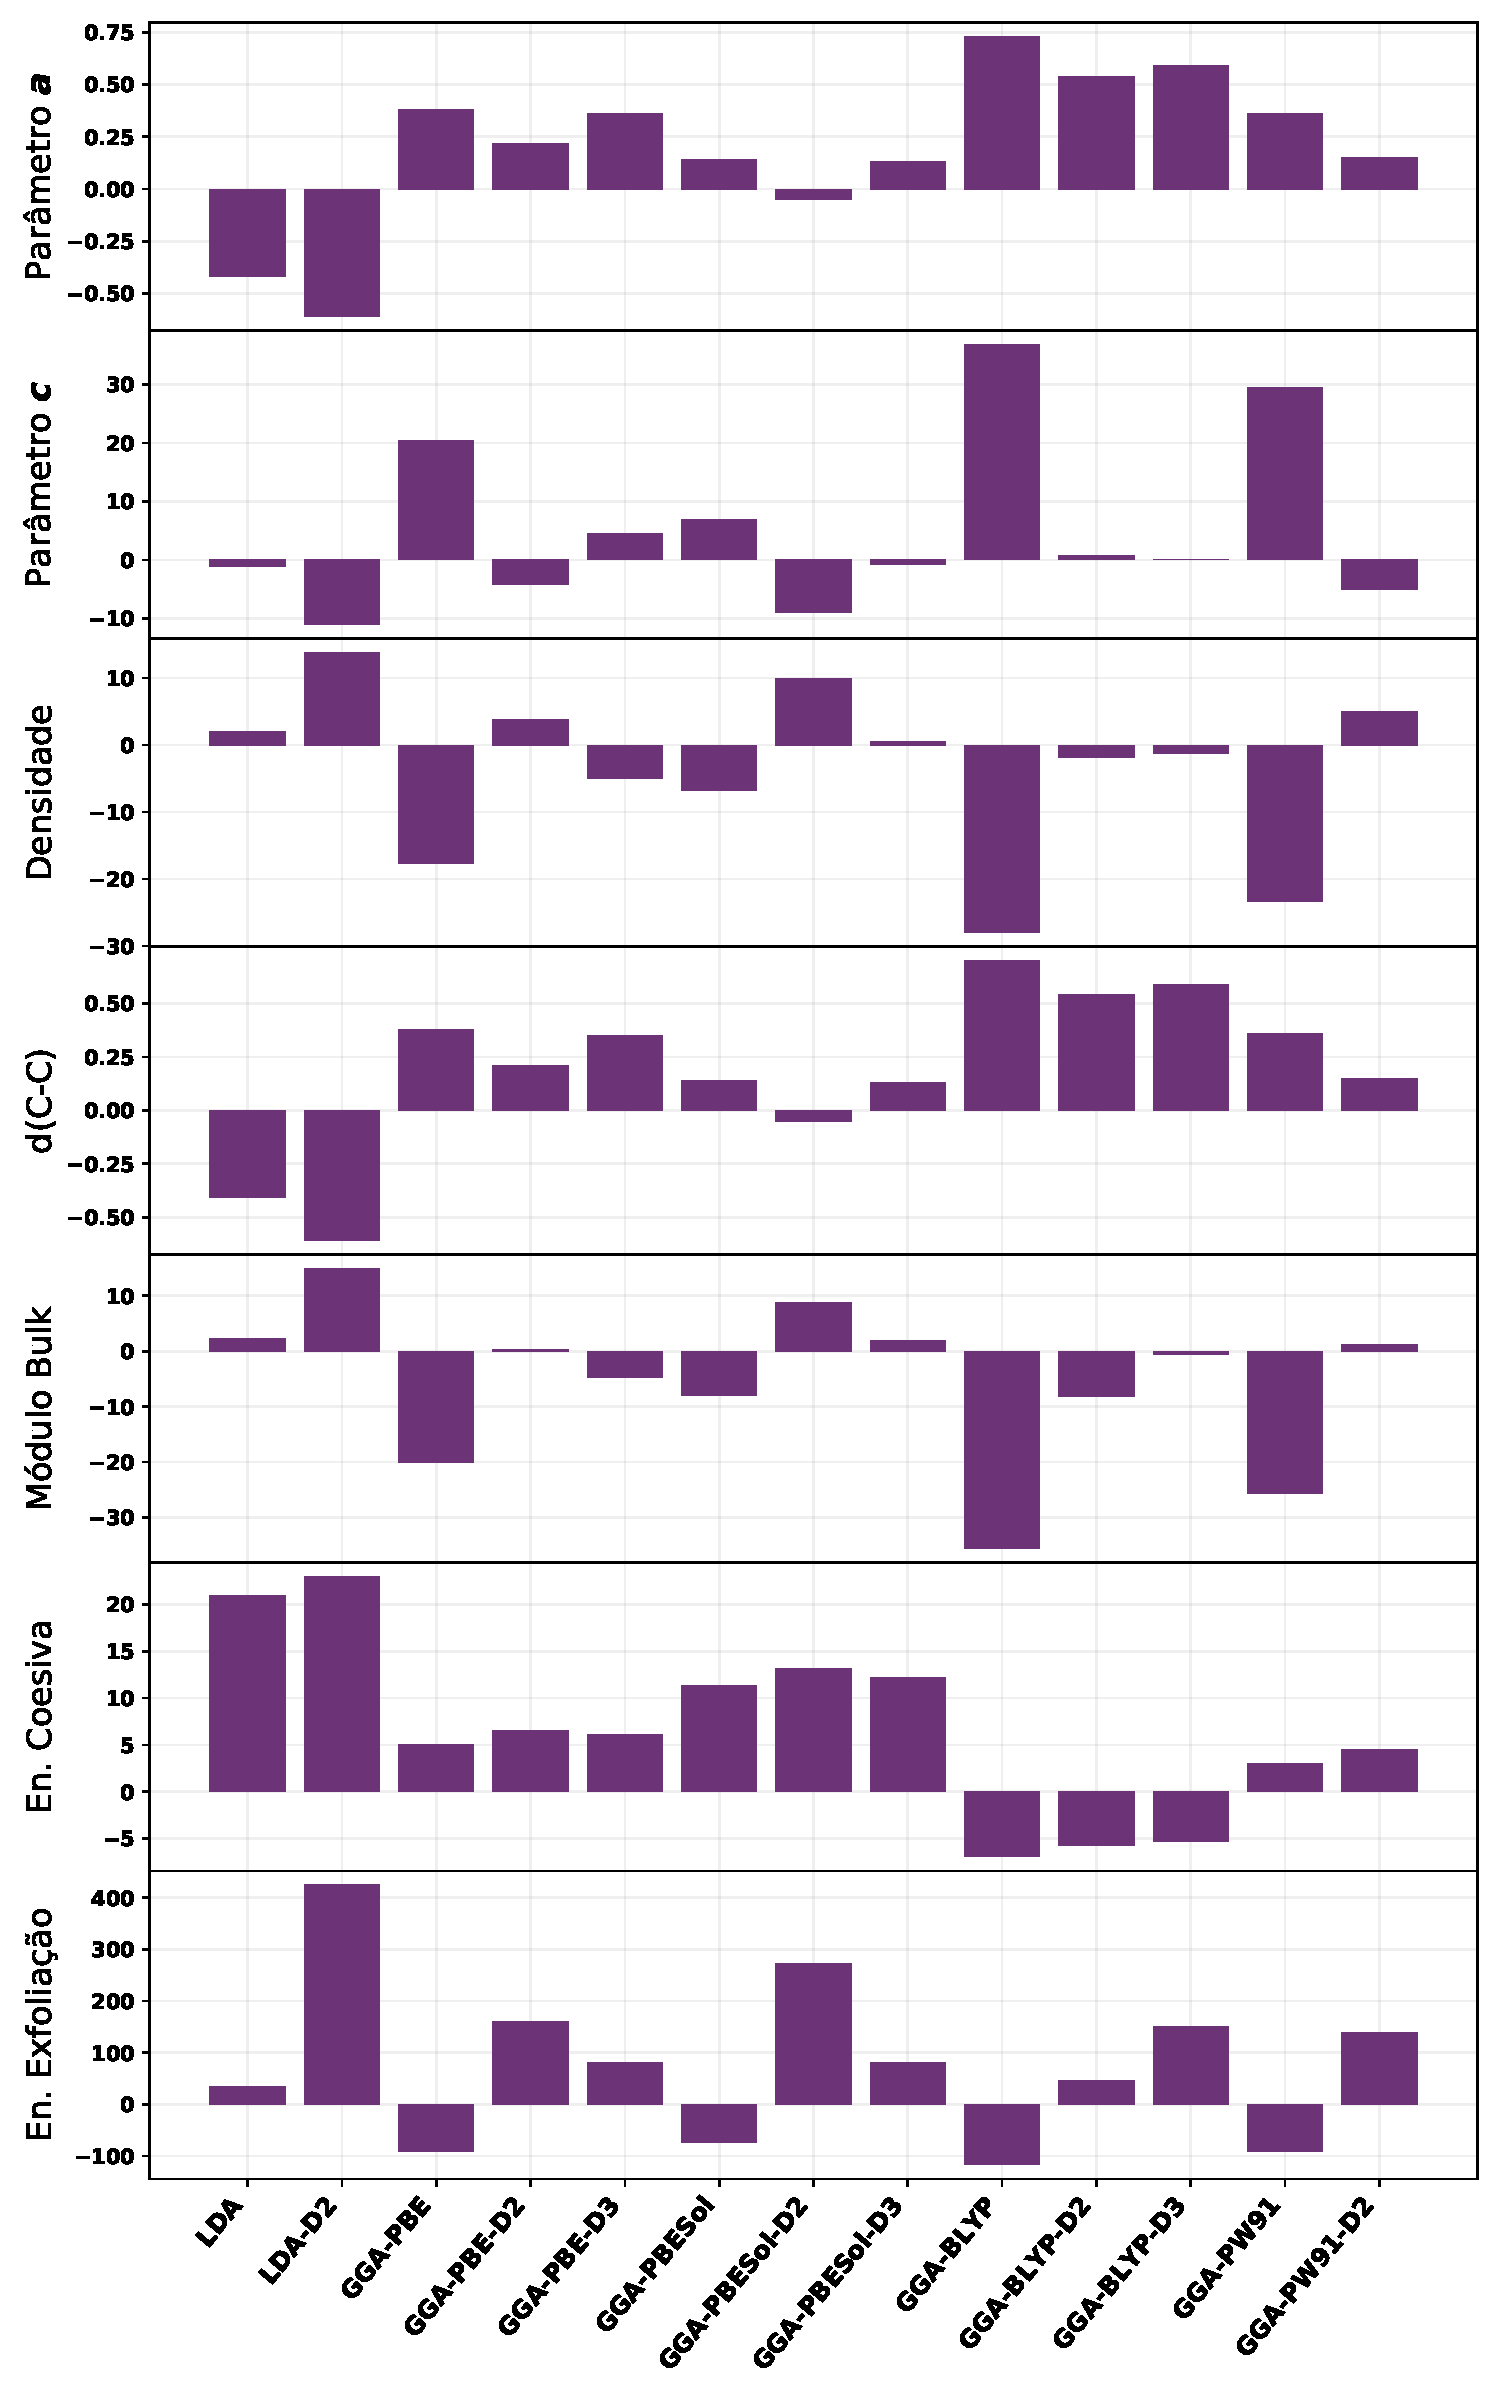
\includegraphics[width=.85\linewidth]{capitulos/fig/results0/disc_rel_grafite}
			\caption{Discrepância relativa percentual de diversas propriedades do grafite calculadas para vários funcionais.}
			\label{disc_rel_grafite}
		\end{figure}
	
		A \autoref{disc_rel_grafite} resume os dados da \autoref{grafite_AB}, representando as discrepâncias relativas entre os valores calculados para os diferentes funcionais e os respectivos valores experimentais. Todos os resultados são relativos à forma alfa. Observando esses resultados é possível notar alguns padrões interessantes. 
		
		O cálculo do parâmetro $a$ da célula unitária mostra que todos os funcionais apresentam bons resultados, tendo o funcional LDA subestimado o valor e os funcionais GGA superestimado os valores. Para o parâmetro $c$ é possível observar que para os funcionais GGA-PBE, GGA-BLYP e GGA-PW91 a correção de Grimme é extremamente importante, pois quando não é utilizada as discrepâncias relativas ficam na casa dos 20\%. Quando a correção de Grimme é utilizada os valores chegam muito mais próximos do experimental, tendo a versão D3 apresentado melhores resultados do que a versão D2 em todos os casos. Curiosamente o funcional LDA foi extremamente bem sucedido sem correção de Grimme, apresentando discrepância relativa de -1.17\%, valor que aumenta para -11.05\% quado a correção de Grimme D2 é utilizada. 
		
		Os valores de comprimento de ligação seguiram o mesmo padrão dos resultados para o parâmetro $a$, uma vez que são diretamente correlacionados. Os resultados para a densidade seguem o mesmo padrão dos resultados para o parâmetro $c$, pois como os valores do parâmetro $a$ são muito próximos do valor experimental, a principal fonte de variação da densidade é o parâmetro $c$. Os resultados para o cálculo do módulo de Bulk seguiram o mesmo padrão da densidade e do parâmetro $c$. 
		
		Para a energia coesiva, podemos observar que o erro do funcional LDA é consideravelmente grande, ficando na casa dos 20\%. O funcional GGA-PBESol apresentou um resultado intermediário, com discrepâncias relativas na casa dos 10\%, seguido pelos funcionais GGA-PBE, GGA-BLYP e GGA-PW91, respectivamente. É interessante ressaltar que o único funcional que apresentou energia coesiva menor que o valor experimental foi o funcional BLYP. 
		
		Para a energia de exfoliação é possível observar que curiosamente o funcional LDA apresentou um ótimo resultado sem correção de Grimme, tendo este piorado muito quando a correção é utilizada. Notadamente os melhores resultados dentre os funcionais GGA forma apresentados por PBE-D3, PBESol-D3 e BLYP-D2. É interessante destacar que o funcional GGA-BLYP apresentou uma energia de exfoliação negativa, indicando que sem correções de Grimme esse funcional falha em prever que o grafite como sólido é mais estável do que com suas folhas separadas (grafeno). 
		
		Como o funcional GGA-PBE-D3 foi o que apresentou, na média, os resultados mais consistentes como os dados experimentais ele foi utilizado para calcular os valores de energias relativas das diferentes fases cristalinas do grafite como apresentados na \autoref{empilhamento_grafite}. Diferença energética entre as fases $\alpha$ e $\beta$ do grafite calculadas nesse nível é de 0.12 kcal/mol, valor muito próximo do experimental de 0.14 $\pm$ 0.04 kcal/mol \cite{greenwood2012chemistry}. Esse resultado mostra que é possível, nesse nível de cálculo, prever a estabilidade relativa entre diferentes fases de um alótropo de carbono tanto de maneira qualitativa, prevendo que a fase $\alpha$ é mais estável que a $\beta$, quando de maneira quantitativa prevendo um valor muito próximo do experimental. 
		
	
	\section{Conclusões}
	
		Neste capítulo foi explorado o desempenho de diversos funcionais para predizer as propriedades dos alótropos de carbono mais conhecidos. Foi possível observar que, em geral, os funcionais GGA apresentaram performance melhor do que o funcional LDA. Dentre os funcionais GGA, o funcional PBE foi o que apresentou resultados mais consistentes para todas as propriedades. 
		
		\begin{figure}[!h]
			\centering
			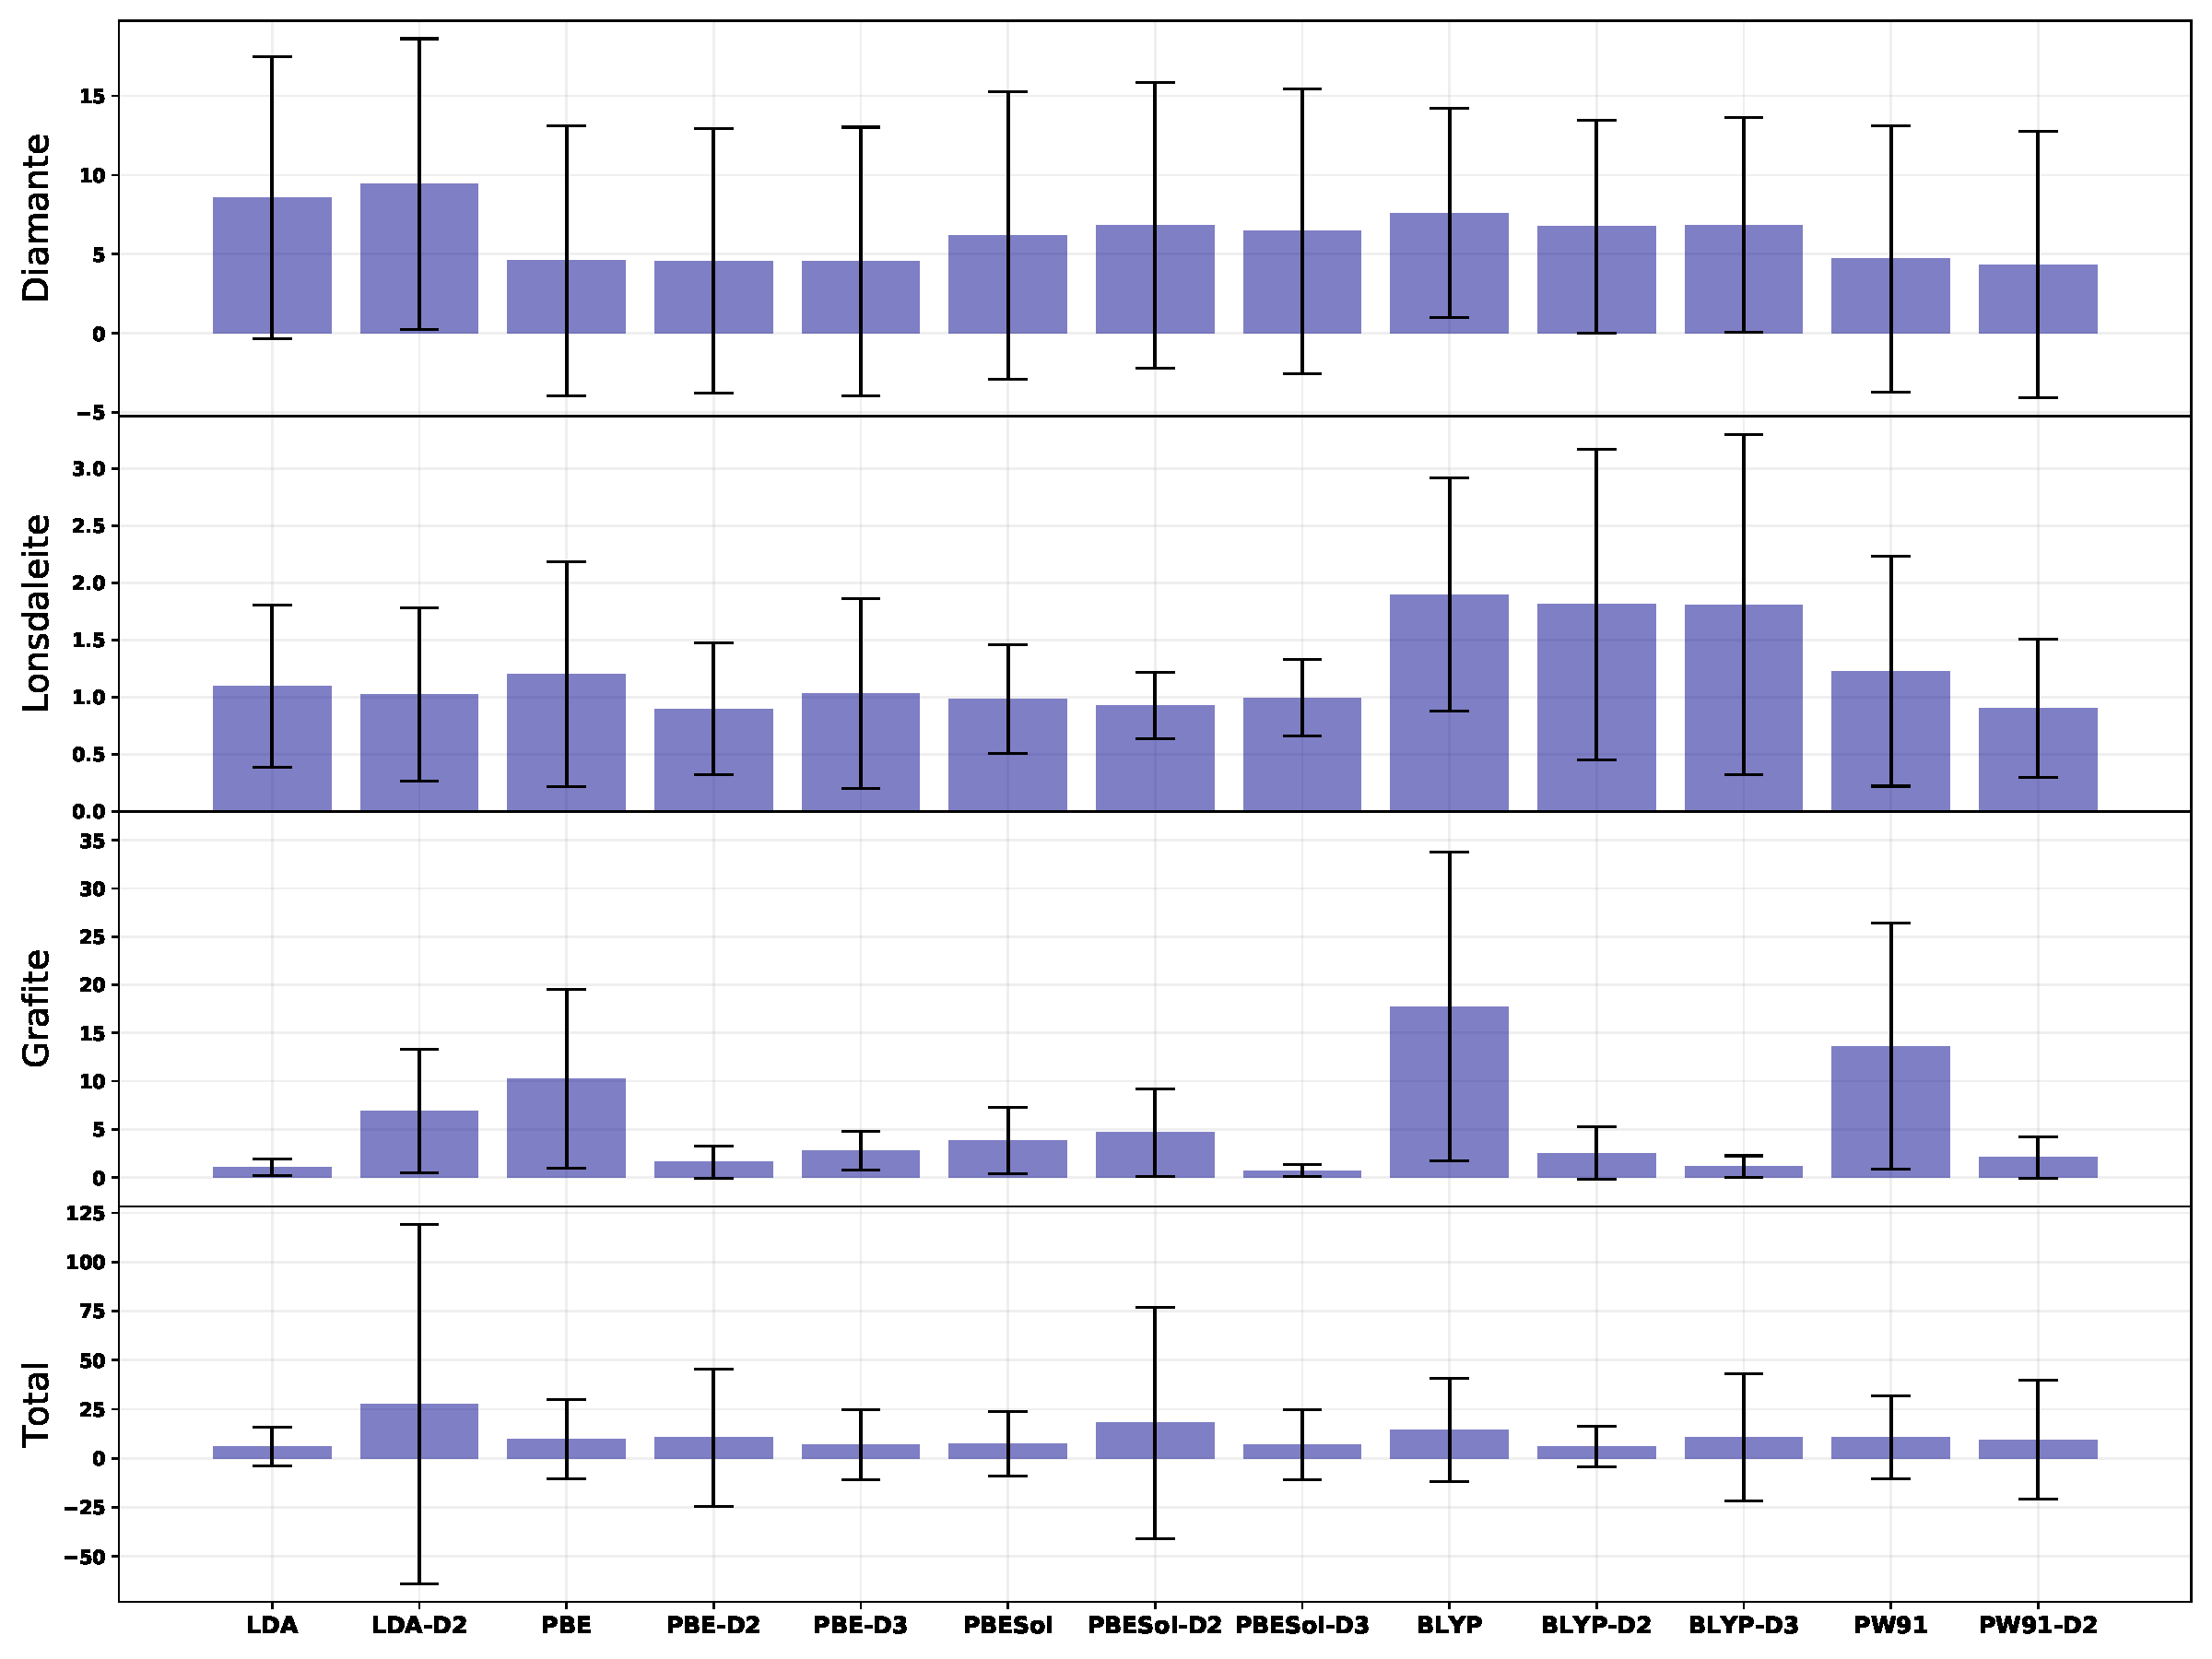
\includegraphics[width=1\linewidth]{capitulos/fig/results0/disc_rel_media}
			\caption{Discrepância relativa percentual média para os três alótropos estudados e a média global.}
			\label{disc_rel_media}
		\end{figure}
		
		Além disso, é possível notar que para o grafite, que apresenta interações do tipo van der Waals entre as folhas, a correção de Grimme é extremamente importante para que se tenha uma estrutura minimamente compatível com os dados experimentais. Curiosamente, entretanto, para o funcional LDA essa correção não foi necessária. Dessa forma, foi escolhido o funcional GGA-PBE-D3 para estudar novas estruturas alotrópicas hipotéticas. 
		
		A \autoref{disc_rel_media} apresenta de maneira concisa a média das discrepâncias relativas, e seus respectivos desvios padrões, para os três alótropos de carbono estudados bem como a média geral para todas as propriedades. 
	
		
	
		
